
\chapter{Memory Forensics}
\newpage

\section{lecture}

\subsection{Evidence}
\begin{itemize}
  \item physical memory
  \item pagefile
  \item crash dumps
  \item hibernation files
\end{itemize}

Memory forensics is critical in digital investigations for several key reasons:

Digital evidence preservation - RAM contains vital volatile data that would be lost if a system is powered down. This includes running processes, network connections, encryption keys, malware artifacts, and system state information that isn't stored on disk.

Malware detection and analysis - Many sophisticated malware variants operate entirely in memory to avoid detection, never writing to disk. Memory forensics can reveal these memory-resident threats, their behaviors, and how they've compromised a system.

Incident response - During active security incidents, memory forensics helps investigators understand what's currently happening on a system, identify unauthorized access, and determine the scope of a compromise without disrupting operations.

Anti-forensics detection - Attackers often use anti-forensics techniques to hide their activities from disk-based investigation tools. Memory analysis can bypass these evasion attempts by examining the actual running state of the system.

Data recovery - Memory can contain recently accessed files, passwords, encryption keys, chat messages, and other sensitive data that may no longer exist on disk. This can be crucial for both criminal investigations and incident response.

Process analysis - Understanding what processes were running, their relationships, loaded modules, and network connections provides investigators with a complete picture of system activity that may not be apparent from disk artifacts alone.

Would you like me to elaborate on any of these aspects of memory forensics?

\begin{quotation}
  maleware can hide, but it has to run
\end{quotation}

\subsubsection*{Artifacts}
\begin{itemize}
  \item processes
  \item network connections
  \item loaded Drivers
  \item console command History
  \item strings in memory
  \item credentials and keys
  \item everything running on a computer
\end{itemize}

\subsubsection*{Windows memory acquisition}
\textbf{Tools}
\begin{itemize}
  \item WinPMEM Rekall
  \item FTK Imager Access Data
  \item FDPro HBGary
  \item Memoryze FireEye
  \item F-Response
\end{itemize}

Sample acquisition using winpmem:

\begin{lstlisting}[language=sh]
C:\> winpmem.exe -0 dump0.raw
\end{lstlisting}

\textbf{Tools:}
\begin{itemize}
   \item AVML (Acquire Volatile Memory for Linux, \url{https://github.com/microsoft/avml})
   \item LiME Linux Memory Extractor
\end{itemize}

\textbf{Profile Generation:}
\begin{lstlisting}[language=sh]
#cd volatility-master/tools/linux
#make -C /lib/modules/<kernel version>/build CONFIG_DEBUG_INFO=y M=$PWD modules
#dwarfdump -di ./module.o > module.dwarf
#zip <servername-kernel-version>.zip module.dwarf /boot/System.map-<kernel-version>
\end{lstlisting}

\textbf{If available as .deb (e.g. Kali)}
\begin{lstlisting}[language=sh]
#apt-get install lime-forensics-dkms
\end{lstlisting}

\textbf{Memory Dump using LiME:}
\begin{lstlisting}[language=sh]
#insmod /var/lib/dkms/lime-forensics/.../module/lime.ko "path=dump.raw format=raw"
\end{lstlisting}



\subsubsection*{Advanced Memory Acquisition Techniques Using DMA}
\begin{center}
  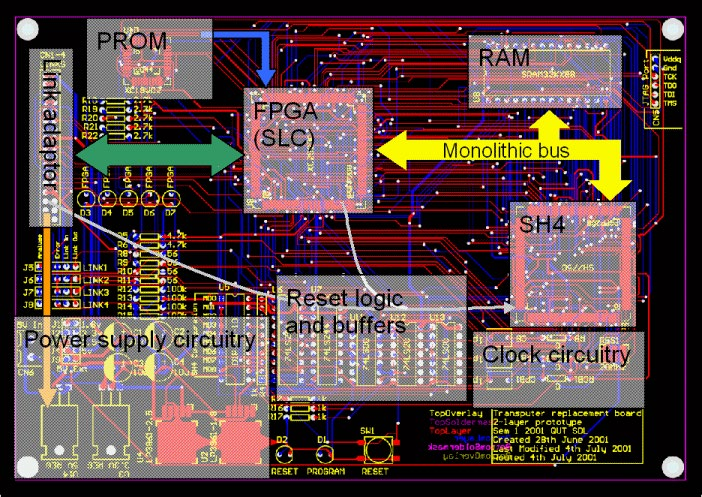
\includegraphics[width=\textwidth]{resources/13-volatility-mainboard.png}
\end{center}

Direct Memory Access (DMA) techniques allow for memory acquisition without using the operating system's APIs or drivers, which helps bypass potential anti-forensics measures. Two notable DMA approaches are:

\textbf{PCIe-based Acquisition}\\
PCI Express (PCIe) enables direct hardware access to system memory through DMA. This technique:
\begin{itemize}
    \item Requires physical access to an available PCIe slot
    \item Can bypass operating system protections
    \item Operates at high speeds due to direct hardware access
    \item Is limited to accessing the first 4GB of RAM due to DMA constraints
\end{itemize}

\textbf{FireWire-based Acquisition}\\
FireWire (IEEE 1394) interfaces also support DMA capabilities. This method:
\begin{itemize}
    \item Uses the FireWire protocol's built-in DMA features
    \item Can acquire memory through a FireWire port without OS interaction
    \item Works cross-platform (Windows, Linux, macOS)
    \item Has the same 4GB memory limitation as PCIe
    \item May require enabling SBP-2 (Serial Bus Protocol 2) support
\end{itemize}

\textbf{Limitations of DMA-based Techniques}
\begin{itemize}
    \item Only access first 4GB of RAM due to 32-bit DMA addressing
    \item Require specialized hardware
    \item Physical access to target system is mandatory
    \item Modern systems may implement IOMMU/VT-d protection
    \item Risk of system instability during acquisition
\end{itemize}

\textbf{Tools for DMA Acquisition}
\begin{itemize}
    \item PCILeech - For PCIe-based acquisition
    \item Inception - FireWire memory dumping tool
    \item WindowsFirewire - Windows-specific FireWire acquisition
\end{itemize}

\subsubsection*{Memory Smear}
\begin{center}
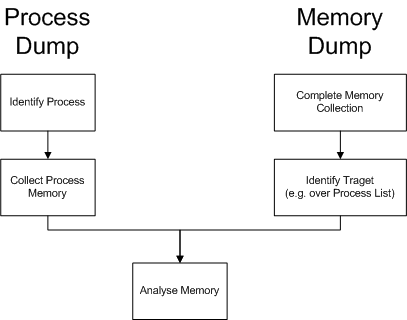
\includegraphics[width=\textwidth]{resources/13-memory-smear.png}
\end{center}

Memory smear is a critical concept in memory forensics that relates to how memory changes during the acquisition process, and this image helps illustrate where it can occur. Let me explain:
Memory smear happens when memory content changes during the acquisition process - imagine trying to take a photograph of a moving object. Just as the photo might be blurry, the memory capture can be "smeared" because the system is still running while you're collecting the memory.

Looking at the diagram:
\begin{enumerate}
  \item In the Process Dump path (left side):
  \begin{itemize}
    \item While you're identifying and collecting process memory, the process is still running
    \item This active state means the process could be modifying memory while you're collecting it
  \end{itemize}
  \item In the Memory Dump path (right side):
  \begin{itemize}
    \item During complete memory collection, the entire system remains active
    \item Other processes continue to run, modifying memory contents
    \item The memory content at the start of collection might be different from the content at the end
  \end{itemize}
  \item Both paths converge at "Analyse Memory" where the impact of memory smear becomes evident:
  \begin{itemize}
    \item You might capture inconsistent data
    \item Process relationships might appear broken
    \item Memory structures might seem corrupted
  \end{itemize}
\end{enumerate}
This is why memory acquisition tools need to be as fast as possible and why some advanced techniques (like DMA approaches we discussed) try to minimize this effect by bypassing the operating system. However, it's important to note that some degree of memory smear is often unavoidable in live systems.


\begin{center}
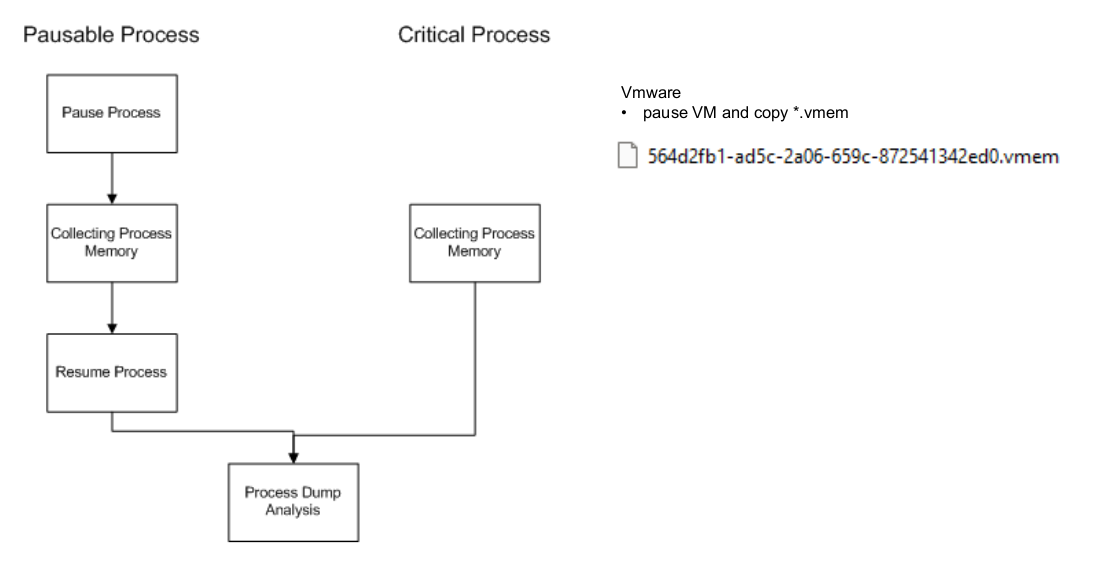
\includegraphics[width=\textwidth]{resources/13-memory-smear-avoid.png}
\end{center}
\textbf{Avoiding Memory Smear in Forensic Memory Acquisition}

There are two primary approaches to avoid memory smear during acquisition, as illustrated in the process flow diagram:

\textbf{1. Pausable Process Approach}\\
This method follows a three-step process:
\begin{itemize}
   \item Initially pauses the target process
   \item Collects process memory while the process is frozen
   \item Resumes the process after collection is complete
\end{itemize}

\textbf{2. Critical Process Approach}\\
For processes that cannot be paused:
\begin{itemize}
   \item Direct memory collection without interruption
   \item Higher risk of memory smear
   \item Required for system-critical processes
\end{itemize}

\textbf{VMware Solution}\\
VMware provides an effective solution using virtual machine capabilities:
\begin{lstlisting}[language=sh]
# Pause VM and copy memory file
vmware-cmd /path/to/vm/file.vmx suspend
cp /path/to/vm/564d2fb1-ad5c-2a06-659c-872541342ed0.vmem /evidence/
\end{lstlisting}

\textbf{Advantages of VMware Approach}
\begin{itemize}
   \item Creates consistent memory state by freezing entire VM
   \item Prevents any process from modifying memory during acquisition
   \item Works for both critical and non-critical processes
   \item Minimal system impact after VM resume
   \item Produces reliable memory dumps without smear effects
\end{itemize}

\textbf{Key Considerations}
\begin{itemize}
   \item Pausable processes: Use suspension when possible
   \item Critical processes: Must use specialized techniques
   \item Virtual environments: Leverage VM suspension capabilities
   \item Time window: Minimize acquisition duration
   \item System impact: Consider operational requirements
\end{itemize}


\subsubsection*{Memory Acquisition Hibernation}
\begin{lstlisting}[language=sh]
 \%SystemDrive\%\\hiberfil.sys 
\end{lstlisting}

\subsubsection*{Memory Acquisition After Crash}
\begin{lstlisting}[language=sh]
 \%WINDIR\%\\MEMORY.DMP
\end{lstlisting}

\subsubsection*{Memory Acquisition Shut Down System}
\begin{lstlisting}[language=sh]
 \%WINDIR\%\\pagefile.sys
 \%WINDIR\%\\swapfile.sys
\end{lstlisting}

pagefile: mostly empty if PC has enough memory
swapfile: Containing Data of Metro Apps

\subsubsection*{Example of process list}

\textbf{PSActiveProcessList}
\begin{itemize}
   \item Double linked List
   \item Process identification via iteration over each element
   \item Used by Windows Task Manager, tasklist or Get-Process cmdlet
\end{itemize}

\begin{center}
  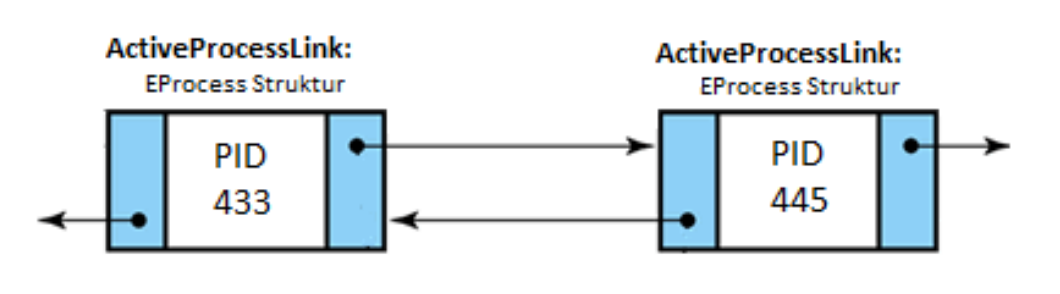
\includegraphics[width=\textwidth]{resources/13-volatility-process-list.png}
\end{center}

\textbf{PSActiveProcessList}
\begin{itemize}
   \item Detaching the process from the linked list hides it from standard tools.
\end{itemize}

\begin{center}
  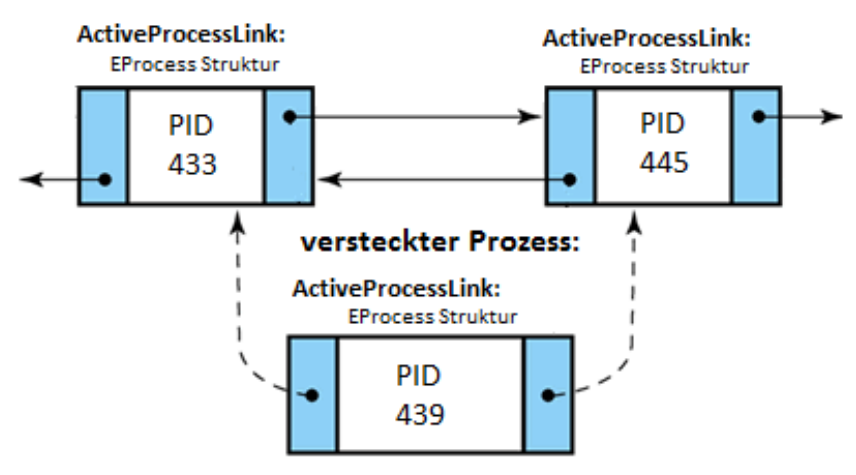
\includegraphics[width=\textwidth]{resources/13-volatility-process-list-2.png}
\end{center}

\subsection{Analysis}
\begin{center}
  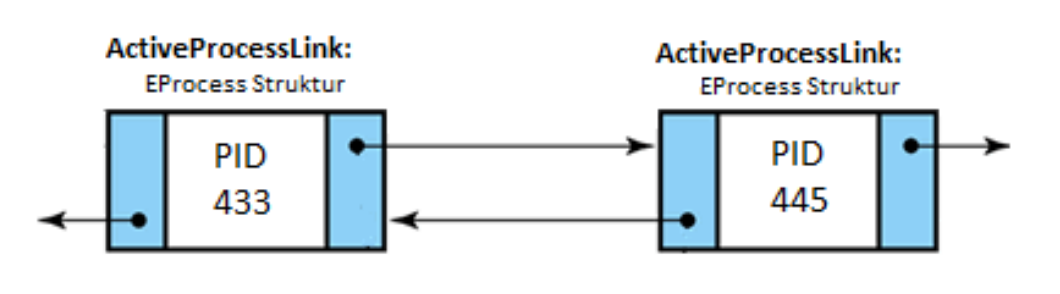
\includegraphics[width=\textwidth]{resources/13-volatility-process-list.png}
  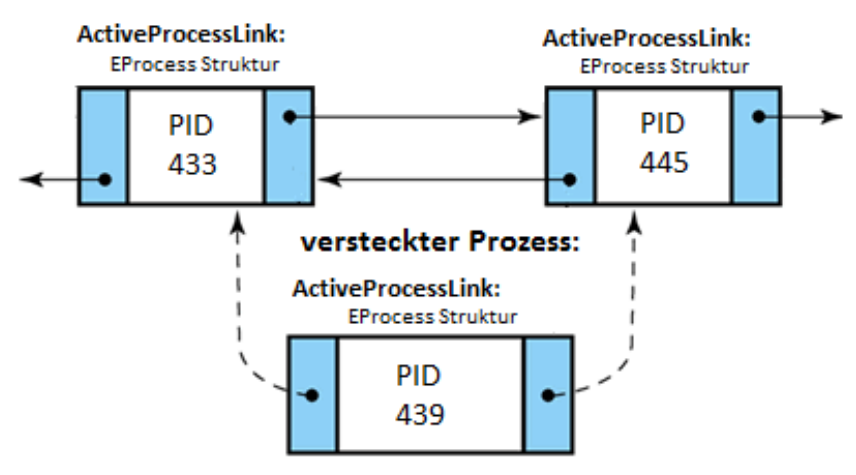
\includegraphics[width=\textwidth]{resources/13-volatility-process-list-2.png}
\end{center}

\begin{itemize}
  \item Redline, Mandiant - commercial
  \item Volatility: free
\end{itemize}
\subsection{Tools}
\textbf{Understanding Volatility Framework}

Volatility is an advanced open-source memory forensics framework that allows investigators to analyze RAM dumps captured from various operating systems. It acts as a digital forensics and incident response (DFIR) tool that can extract artifacts from volatile memory, providing crucial information about the system's state at the time of capture.

\textbf{Key Features of Volatility}
\begin{itemize}
   \item Cross-platform analysis (Windows, Linux, macOS)
   \item Extensible plugin architecture
   \item Support for multiple memory dump formats
   \item Advanced memory artifact recovery techniques
   \item Comprehensive process and thread analysis
   \item Registry parsing and analysis
   \item Network connection investigation
\end{itemize}

\textbf{Version Differences}\\
Volatility 2 vs Volatility 3:
\begin{itemize}
   \item \textbf{Volatility 2}
       \begin{itemize}
           \item Written in Python 2.7
           \item Requires specific profiles for analysis
           \item More plugins available due to longer existence
           \item Complex profile management
           \item Slower analysis speed
       \end{itemize}
   \item \textbf{Volatility 3}
       \begin{itemize}
           \item Written in Python 3
           \item Automatic OS detection without profiles
           \item Symbol tables replace traditional profiles
           \item Improved performance and speed
           \item More modern codebase and architecture
           \item Better handling of large memory dumps
       \end{itemize}
\end{itemize}

\textbf{Alternatives to Volatility}
\begin{itemize}
   \item \textbf{Rekall}
       \begin{itemize}
           \item Fork of Volatility
           \item Focus on live memory analysis
           \item Integrated with Google Cloud
       \end{itemize}
   \item \textbf{WindowsSCOPE}
       \begin{itemize}
           \item Commercial solution
           \item Real-time memory analysis
           \item Windows-specific features
       \end{itemize}
   \item \textbf{Memoryze}
       \begin{itemize}
           \item By FireEye/Mandiant
           \item Free but closed-source
           \item Windows memory analysis focus
       \end{itemize}
\end{itemize}

\textbf{Installation on Linux}\\
Multiple installation methods are available:

\begin{lstlisting}[language=sh]
# Method 1: Using pip
pip3 install volatility3

# Method 2: From source
git clone https://github.com/volatilityfoundation/volatility3.git
cd volatility3
python3 setup.py install

# Method 3: Using virtual environment (recommended)
python3 -m venv volatility3-env
source volatility3-env/bin/activate
pip3 install volatility3
\end{lstlisting}

\textbf{Basic Usage Examples}\\
Common analysis scenarios:

\begin{lstlisting}[language=sh]
# List all available plugins
vol -h

# Analyze Windows memory dump
vol -f memory.dump windows.info        # System information
vol -f memory.dump windows.pslist      # Process listing
vol -f memory.dump windows.netscan     # Network connections
vol -f memory.dump windows.filescan    # File handles
vol -f memory.dump windows.malfind     # Detect injected code

# Analyze Linux memory dump
vol -f memory.dump linux.bash          # Bash history
vol -f memory.dump linux.pslist        # Process listing
vol -f memory.dump linux.lsmod         # Loaded modules

# Advanced Analysis
vol -f memory.dump windows.registry.printkey --key "Software\Microsoft\Windows\CurrentVersion\Run"
vol -f memory.dump windows.dlllist --pid 1234
vol -f memory.dump windows.handles --pid 1234
\end{lstlisting}

\textbf{Use Cases in Digital Forensics}
\begin{itemize}
   \item \textbf{Incident Response}
       \begin{itemize}
           \item Analyzing active malware infections
           \item Identifying unauthorized processes
           \item Investigating network connections
           \item Detecting rootkits and hidden processes
       \end{itemize}
   \item \textbf{Malware Analysis}
       \begin{itemize}
           \item Code injection detection
           \item Memory-resident malware discovery
           \item Process hollowing identification
           \item Rootkit detection
       \end{itemize}
   \item \textbf{Digital Investigation}
       \begin{itemize}
           \item Password recovery
           \item Encryption key extraction
           \item Browser history analysis
           \item Command history reconstruction
       \end{itemize}
\end{itemize}

\section{exercise}
